\documentclass[a4paper]{article}
\usepackage[utf8]{inputenc}
\usepackage[T1]{fontenc}
\usepackage{cite}
\usepackage{graphicx}
\usepackage{hyperref}

\iffalse
1) Le contexte, la problèmatique, les contributions de l’article choisi (2 pages environ)
2) Le plan d’expérience que vous comptez mener, les données que vous comptez utiliser (2 pages max).
\fi

\title{Projet AS : WaveNet}
\author{Seurin Mathieu}

\begin{document}

\maketitle

\section{WaveNet : Génération de son}

Le but de WaveNet \cite{DBLP:journals/corr/OordDZSVGKSK16}, à la base, est de faire de la génération de son brut et plus particulièrement la génération de voix humaine (on verra que WaveNet va plus loin). L'idée est simple, le programme reçoit en entrée un texte, et le but est de faire sortir une voix la plus réalise possible, récitant le texte. Cette tâche s'appelle de la synthèse vocal ou TTS (Text-To-Speech).

Il existe deux concurrents actuellement et c'est avec eux que WaveNet est comparé. Le premier s'appelle 'concatenative TTS' (méthode par concatenation) et le deuxième 'parametric TTS' (méthode paramétrique). La méthode par concatenation utilise pleins d'enregistrements de voix et les 'colle' bout à bout pour générer le discours mis en entrée. Le processus fonctionne relativemment bien mais il a ses limites. L'enregistrement est coûteux car il faut le faire pour chaque mot (et rajouter un mot nécessite un nouvel enregistrement) et l'enregistrement doit être très precis (même timbre de voix, même vitesse de parole, même volume etc ...). De plus, ajouter une nouvelle voix oblige à ré-enregistrer tout. La deuxième méthode est paramétrique : Au lieu de coller des enregistrements de mots, le discours va être généré par le modèle. Les premiers sont des modèles dits de vocodeur, où on va appliquer plusieurs filtres sur un signal pour simuler l'appareil vocal d'un humain et donc simuler une voix.
Les deuxièmes sont des modèles qui auront appris sur une base de voix humaine (WaveNet rentrent dans cette catégorie, de modèles appris sur de la voix humaine). Classiquement ces modèles sont à base de chaines de Markov.

La problématique est d'obtenir un son de voix qui est le plus naturel possible et avoir des modèles flexibles. Les modèles par concatenation sonnant relativement bien, parfois un peu haché, mais ils ne sont pas du tout flexible. Actuellement les modèles paramétriques sont plus flexible, mais sonne moins naturel que les méthodes par concatenation.
L'objectif de WaveNet est donc de créer un modèle paramétrique flexible et qui soit au moins aussi bon que des modèles par concatenation.

\section{L'approche de WaveNet}

L'approche WaveNet est celle d'un modèle paramétrique, avec base d'apprentissage. Pour le moment, la littérature est centrée sur des modèles RNN et LSTM \cite{DBLP:journals/corr/ZenAEHS16}., mais on trouve également des modèles Markoviens \cite{zen2009statistical}.

L'approche WaveNet est à base de réseaux de neurones convolutifs causaux dilatés. Nous allons expliquer le principe plus en détails.

Le but est de générer un signal d'environ 16000 échantillons à la seconde, chaque échantillon dépendant des échantillons précédents (on verra dans quel mesure).
L'architecture proposée n'est pas à base de RNN mais de réseaux de convolutions causaux, ce qui veut dire que l'output $x_t$ (échantillon $x$ au temps $t$) va être la résultante de filtres de convolution appliqués au $x_k ... x_{t-1}$ avec $k<t$ (voir \autoref{fig:SimpleModel}, où sont utilisées 3 couches de convolution pour illustrer, dans la réalité, il y a bien plus de couches et les filtres sont plus gros)

\begin{figure}[h]
  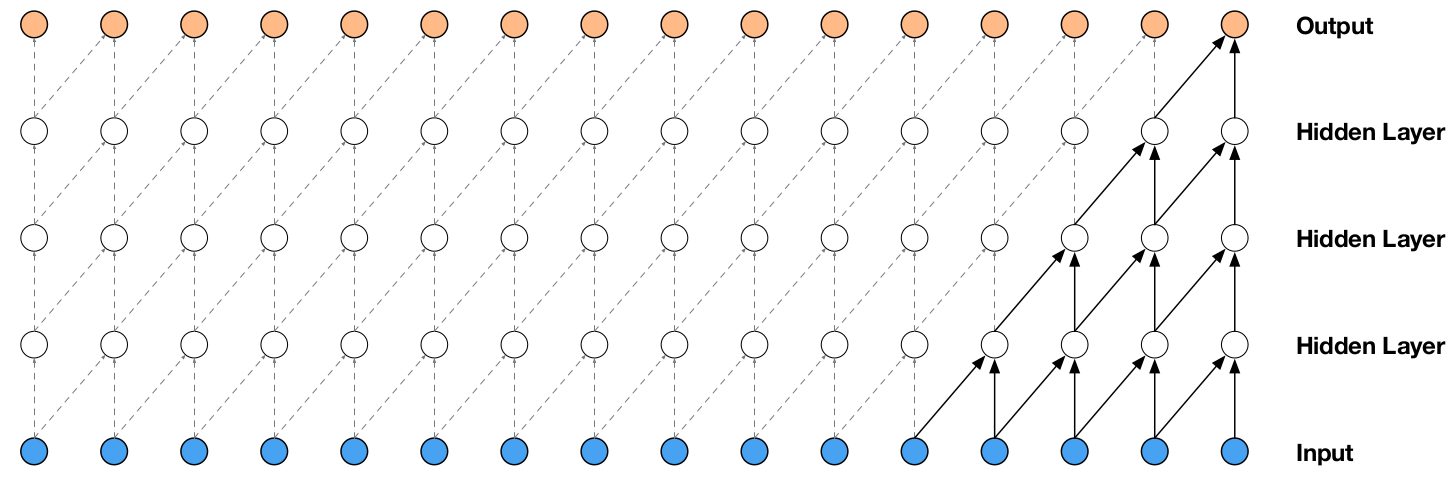
\includegraphics[scale=0.2]{modelSimple.png}
  \caption{\label{fig:SimpleModel} Réseaux de convolutions causaux}
\end{figure}

Le principal problème de cette architecture est qu'elle a besoin d'énormément de couches (combinaisons de plusieurs filtres) et de filtres gros (= qui filtrent beaucoup de pas de temps et qui remonte loin dans le passé), cela pose donc un problème niveau temps/coût de calcul.

Pour remédier au deuxième problème, les auteurs utilisent une structure différente : Les CNN causaux dilatés. Le principe est illustré sur la \autoref{fig:modelDilate}. Le but est d'augmenter la taille des filtres des couches cachées mais sans décupler le nombre de calcul à effectuer. Cela permet aux filtres des couches cachés de récupérer de l'infos de pas de temps plus éloignés.

Plus l'on va dilater un filtre, plus il va capter l'information de pas temps éloignés. Attention, un fitre trop dilaté risque de 'sauter' des pas de temps et d'ignorer les échantillons récents, ce qui n'est pas un comportement voulu.

\begin{figure}[h]
  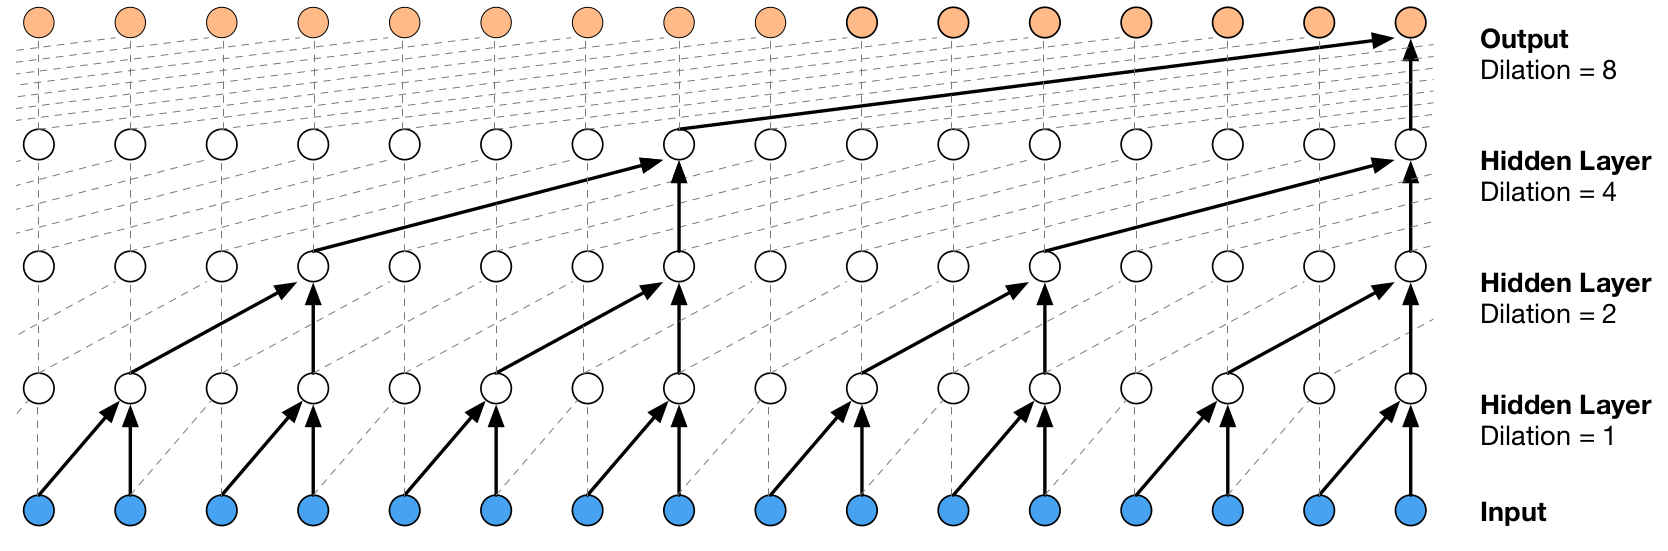
\includegraphics[scale=0.2]{modelDilate.png}
  \caption{\label{fig:modelDilate} Réseaux de convolutions causaux}
\end{figure}

\section{Expériences mises en place}

L'application de WaveNet est évidemment la génération de voix humaine, mais nous avons détourné son utilisation pour en faire un générateur de musique midi. WaveNet permet de générer du son mais représente 60h de base d'entrainement, apprise pendant plusieurs semaines sur (multiples) GPU. Il génère 16 000 échantillons à la seconde (et cela prend 90 minutes pour générer une seconde de son), tous ces chiffres pour dire : Générer du son, c'est une structure hors-norme et donc impossible à reproduire sans des moyens. Donc, on va générer de la musique (car même si le tempo est élevé, il y rarement plus de 15 notes à la seconde)

\subsection

\bibliography{SeurinRapport}
\bibliographystyle{apalike}
\end{document}
